\chapter{Brief introduction to sciences using neutrons}
\chaptermark{Brief introduction to sciences using neutrons}
\cleardoublepage

\minitoc

\section{Introduction}
\begin{refsection}
  \label{ch1:Introduction}
  This chapter presents the general context behind the European Spallation Source. In facts, this thesis has almost nothing related to neutron science and this chapter only serves as a quick overview of the different themes in neutron science in order to answer the following question: Why building an 1.8 billion € neutron source is crucial for sciences?

  After a brief historical review about neutron, this chapter presents what a is neutron and why its properties are interesting for probing matter and structures. A concrete application of neutron sciences including usage for different domains will be illustrated. Finally, the different ways of producing a neutron are also briefly presented as well as the advantages and drawbacks of each method.

  \section{History}
  \cite{Chadwick1932}

  \section{Neutron and neutron interaction with matter}
  \label{ch1:sec:Neutron}
  A neutron is a non-elementary particle with no charge. Its mass is $939.56\,\mathrm{MeV/c^{2}}$ ($1.67 \cdot 10^{-27}\,\mathrm{kg}$). A neutron does not have strong electromagnetic interaction with the electron of atoms, unlike charged particles or photon. Therefore, neutrons can travel long distances without major interaction. The neutron has a spin of $\frac{1}{2}$ and a low magnetic moment. Therefore it is possible to polarize a neutron beam. The magnetic moment allows it to interact with magnetic fields in the structures of matter. A neutron interacts mainly with the elements of the nucleus through strong interactions. A free neutron has a lifetime of $881.5\,\mathrm{s}$ and decays into a proton, an electron, and an antineutrino.
  Neutrons follow the principle of wave-particle duality. They can therefore be studied both as a particle and as a wave. Neutrons can be distinguished by their energies, velocities or wavelengths:

  \begin{equation*}
    E_{neutron} = \frac{h^{2}}{2m_{neutron}\lambda^{2}}
  \end{equation*}

  There are several ranges with more or less arbitrary limits:

  \begin{table}[ht]
  \centering
  \caption[Neutron classification according to the neutron energy and wavelength]
  {Neutron classification according to the neutron energy and wavelength. Different sources report different conventions. The range  limits here presented are taken from \cite{psiNeutronRange}.}
  \label{chap1:tab:neutronsT}
  \begin{tabularx}{\linewidth}{lXXX}
    \toprule
    Characteristic        & Energy               & Speed                              & Wavelength                                    \\
    \midrule
    Fast neutrons         & $>1\,\mathrm{MeV}$   & $>1.38\cdot 10^{7}\,\mathrm{m/s}$  & $>2.86\cdot 10^{-4}\,\mathrm{\si{\angstrom}}$ \\
    Intermediate neutrons & $>1\,\mathrm{eV}$    & $>1.38 \cdot 10^{4}\,\mathrm{m/s}$ & $>0.28\,\mathrm{\si{\angstrom}}$              \\
    Epithermal neutrons   & $>100\,\mathrm{meV}$ & $>4.37 \cdot 10^{3}\,\mathrm{m/s}$ & $>0.9\,\mathrm{\si{\angstrom}}$               \\
    Thermal neutrons      & $>12\,\mathrm{meV}$   & $>1.51 \cdot 10^{3}\,\mathrm{m/s}$ & $>0.28\,\mathrm{\si{\angstrom}}$              \\
    Cold neutrons         & $>0.12\,\mathrm{meV}$ & $>151\,\mathrm{m/s}$               & $>26\mathrm{\si{\angstrom}}$                  \\
    Ultra cold neutrons   & $<300\,\mathrm{neV}$ & $<6\,\mathrm{m/s}$                 & $<500\,\mathrm{\si{\angstrom}}$               \\
    \bottomrule
  \end{tabularx}
\end{table}


  Fast neutrons can be slow down precisely with the help of moderators. These moderators are mainly composed of light elements. Indeed in the energy loss of by neutron due elastic scattering with light elements is important. The most common moderators are hydrogen, water, heavy water and graphite.


  \section{Neutronic science, applications and perspective}
  
  \begin{figure}[!ht]
	\begin{center}
		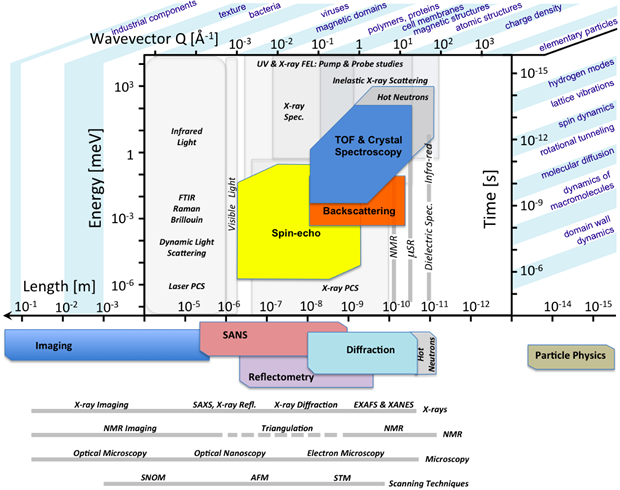
\includegraphics[width=\textwidth]{01_Introduction/figures/fig000_Time_Scale}
	\end{center}
	\caption[Ranges of distances and times of existing neutron scattering techniques]{Ranges of distances and times of existing neutron scattering techniques \cite{essNeutronProbe}.}
	\label{chap1:fig:Time_Scale}
\end{figure}


  \section{Neutron production}
  Producing neutrons is not a trivial task compared to producing charged particles or even photons. The following sections present the principle of operation of thermal neutron user facilities. The term user facilities means that the installation must be open for external user from various scientific domains. Facilities dedicated to specific measurements using neutrons (thermal or non-thermal) are not considered.
  %Obviously, the list is not exhaustive and complete review of existing 

  \subsection{Sources and composite sources}



  \subsection{Nuclear reactors}
  An Uranium 235 atom splits into two lighter nuclei under the impact of a neutron. The fission reaction also lead to neutron emission and energy release:
  \begin{equation*}
    _{92}^{235}U + _{0}^{1}n \rightarrow _{92}^{236}U^* \rightarrow X + Y + k \times _{0}^{1}n
  \end{equation*}
  with X and Y of the fission fragments and k the number of neutrons released during the fission reaction. The neutrons are thermalized in order to increase the probability of further fissions on other Uranium 235 atoms and create chain reaction. In average, each fission of Uranium 235 atoms generates around 2.5 neutrons.

  The fission reaction is the basis of nuclear power plants and research reactors used to produce neutrons.
  Currently, it is the most widely used method used to produce steady state intense neutron beam. The moderation of neutrons is done directly in the pool.
  Some reactor can work in pulsed mode but it is not straightforward and it more efficient to use neutron chopper.

  About ten research reactors open for users are open in Europe, two of them are located in France:
  \begin{itemize}
    \item The Institut Laue-Langevin (ILL): an international facility based on a 58 MW high flux reactor.
    \item The Léon Brillouin Laboratory (LLB): a national facility based on a 14 MW high flux reactor.
  \end{itemize}
  The number of unique users of these two facilities represents one third of the total number for all European neutron facilities.

  Fusion reactions also produce neutrons, but current technology does not allow exploitation as a neutron source.

  \subsection{Spallation sources}
  The term spallation defines the process of neutrons production by bombarding a target with energetic heavy particles (protons, deuterons, neutron etc.). The description of this model was proposed by Saber in 1946 \cite{PhysRev.72.1114}. The process takes place in two stages. When the incident particle has sufficient energy, typically between $100\,\mathrm{MeV}$ and a few GeV, it can interact with several nucleons of a nucleus per intranuclear cascade. In this process nucleons are ejected from the nucleus. After a cascade, the nucleus is in an excited state that can lead to several forms of de-excitation: mainly fissions or evaporation of light elements. Fig. \ref{chap1:fig:spallation} illustrates the spallation process.

  \begin{figure}[!ht]
	\begin{center}
		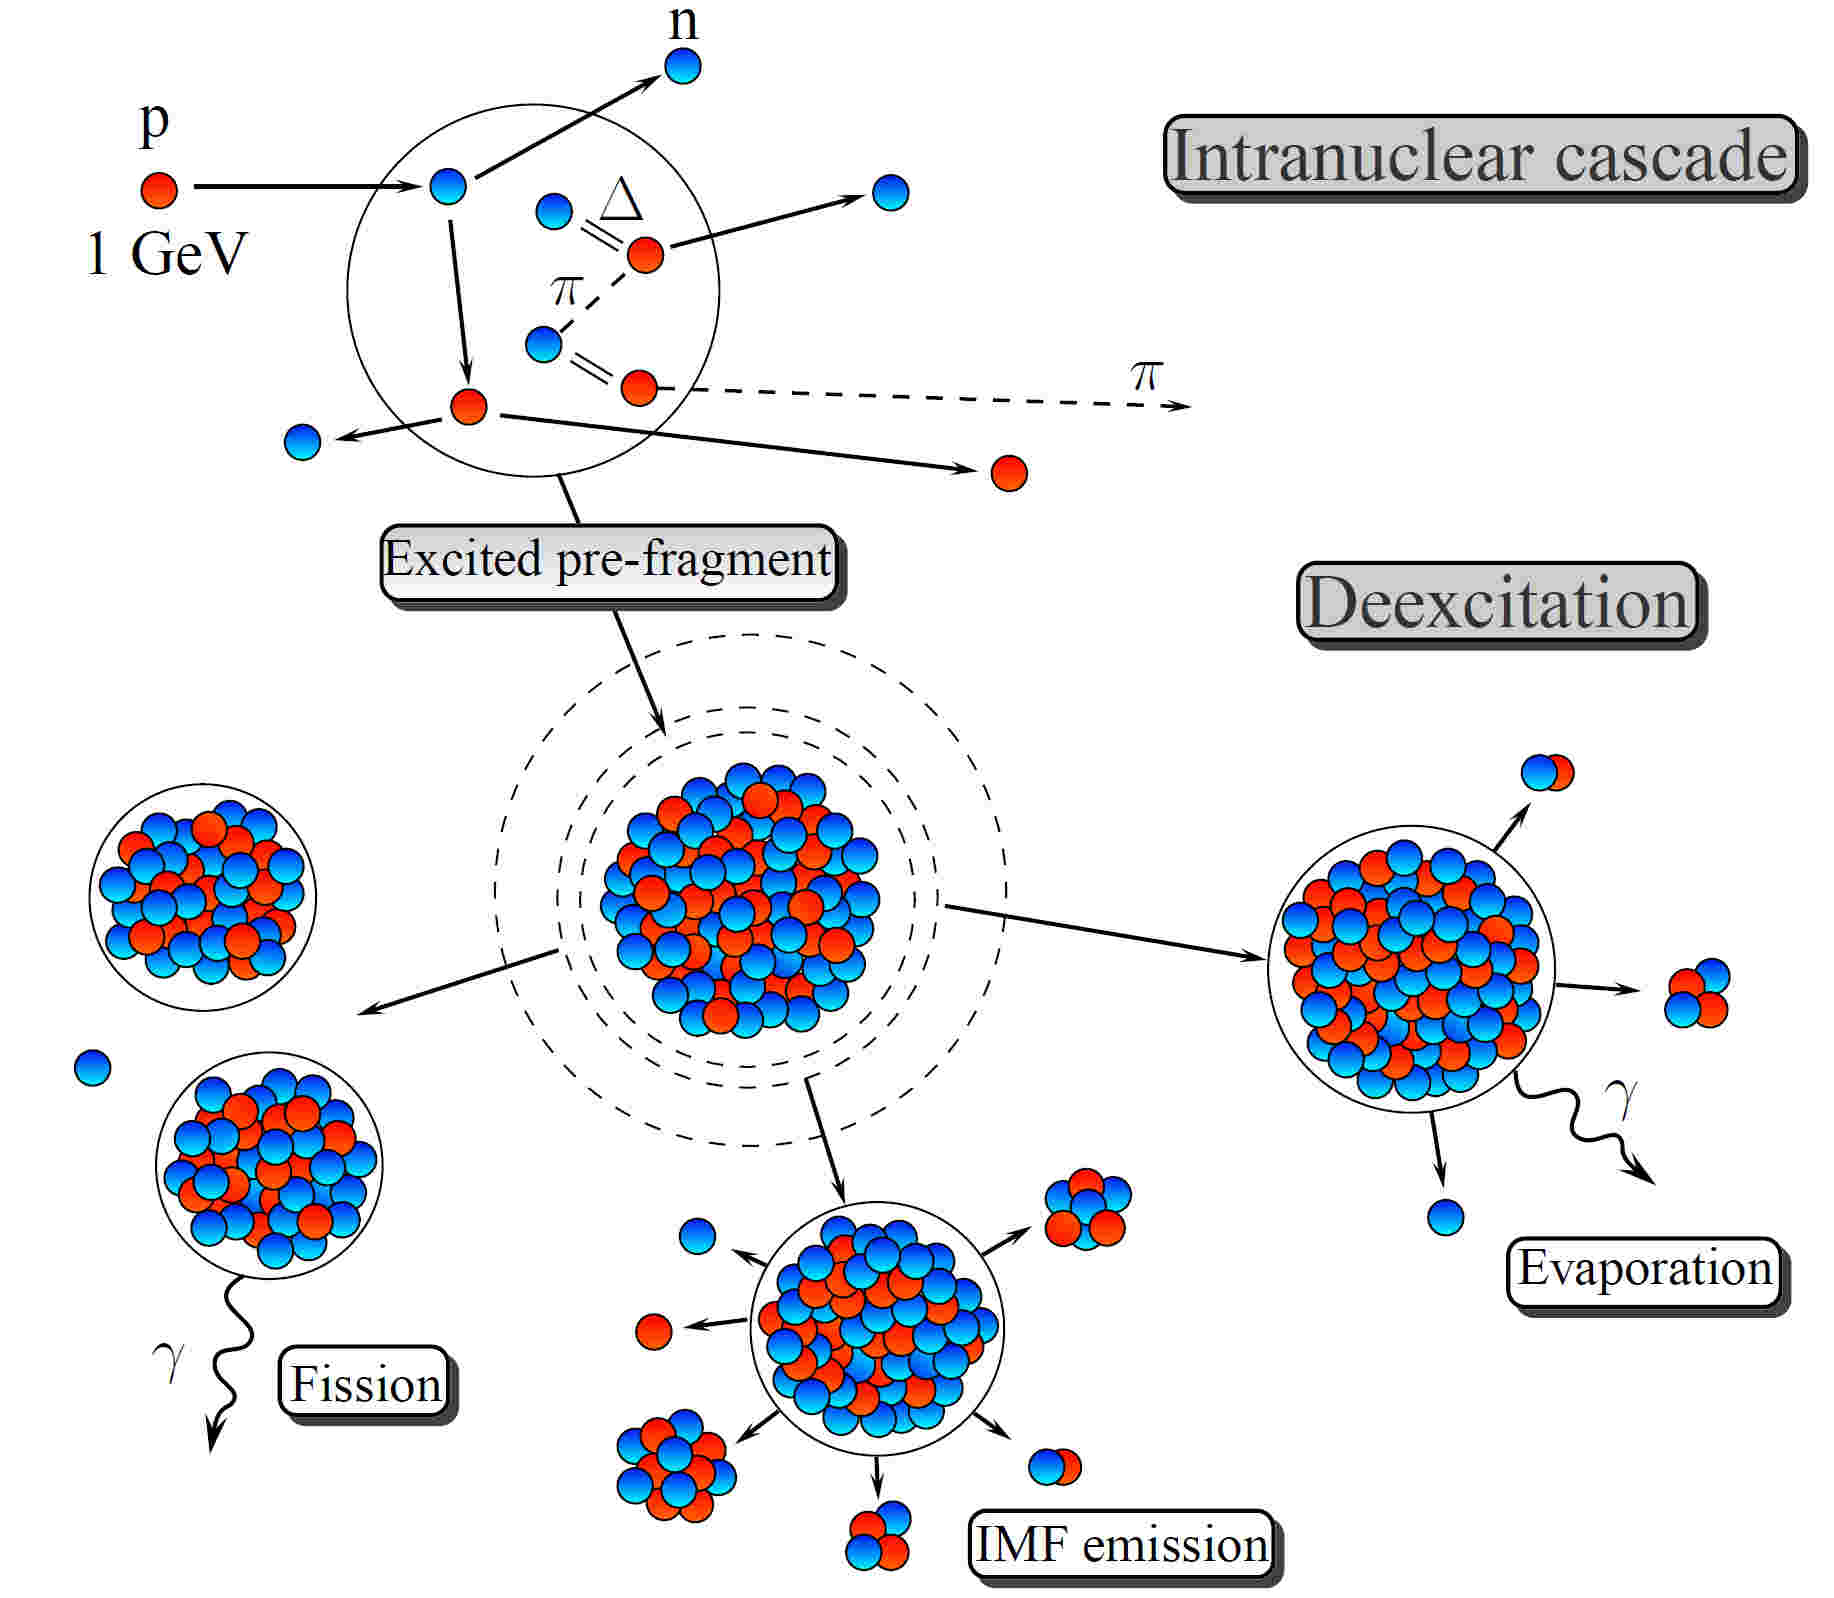
\includegraphics[width=\textwidth]{01_Introduction/figures/fig000_spallation}
	\end{center}
	\caption[Schematic view of the spallation process.]{Schematic view of the spallation process \cite{gorbinet:tel-00660583}. The incident proton interact with nucleons of the target nucleus. An intranuclear cascade occurs leaving the target atom at excited state. Depending of property of the excited nucleus different de-excitation process may occur.}
	\label{chap1:fig:spallation}
\end{figure}


  The neutrons are generated in a wide spectrum whose maximum energy is slightly below the energy of the incident particle energy. The number of neutrons produced by spallation depends on the properties of the target and the incident particle. By choosing a dense target the probability of interaction can but maximized. A dense material also stops most of the emitted particles except gamma and neutrons. The most popular materials are Tungsten, Lead and Mercury as well as actinides\footnote{Actinides should be avoided because they lead to unwanted fissions}. The optimal energy to trigger spallation reactions is between $2\,\mathrm{GeV}$ and $5\,\mathrm{GeV}$.

  A spallation neutron source uses accelerator and a target to produce neutrons following the process described above. A spallation source is totally controlled by its accelerator, allowing to produce intense neutron pulse. It is therefore a complementary method to the research reactor that provide only a continuous flux.

  The first studies of this type of source were carried out in the early 1970s and the first generation sources were built in the 1980s \cite{Klein}. In Europe the first major spallation source was ISIS inaugurated in 1985 \cite{THOMASON201961}. These sources met success and a new generation of spallation sources has been considered. The second generation sources were achieved in 2000-2010 with \acrshort{sns} \cite{Mason2005}, \acrshort{jsns} \cite{Ikeda2002} and \acrshort{csns} \cite{Chen2016}. However, no major second-generation source has been built in Europe.

  \section{The need of a European Spallation Source}
  \label{ch1:Summary}
  Neutrons are a popular tool in the European scientific community and for a long time Europe was a leader in neutron production. However, the future does not look so good with a decrease of the time access on neutron lines for scientists. These are the conclusions of an European Strategy Forum on Research Infrastructures (ESFRI) report in 2016 \cite{neutron2016}.

  The majority of neutron sources is based on reactors built before the 1980s.
  The LLB reactor is years old wheras ILL reactor diverged in . In Europe, despite the success of ISIS\footnote{ISIS was supposed to operate during 20 years but is still running after 35 years.} and SINQ, no second generation neutron source like SNS has been built. At same time, only few new reactors have been built in recent years. Most of neutron source have to be closed within less than 20 years.

  The European Spallation Source (ESS) is project of a intense pulsed neutron source. ESS is a crucial project to maintain the level of expertise of neutron users in Europe and to stimulate a renewal in neutron production, whether through new research reactors or accelerator-driven sources.

  \begin{figure}[!ht]
	\begin{subfigure}[t]{0.5\textwidth}
		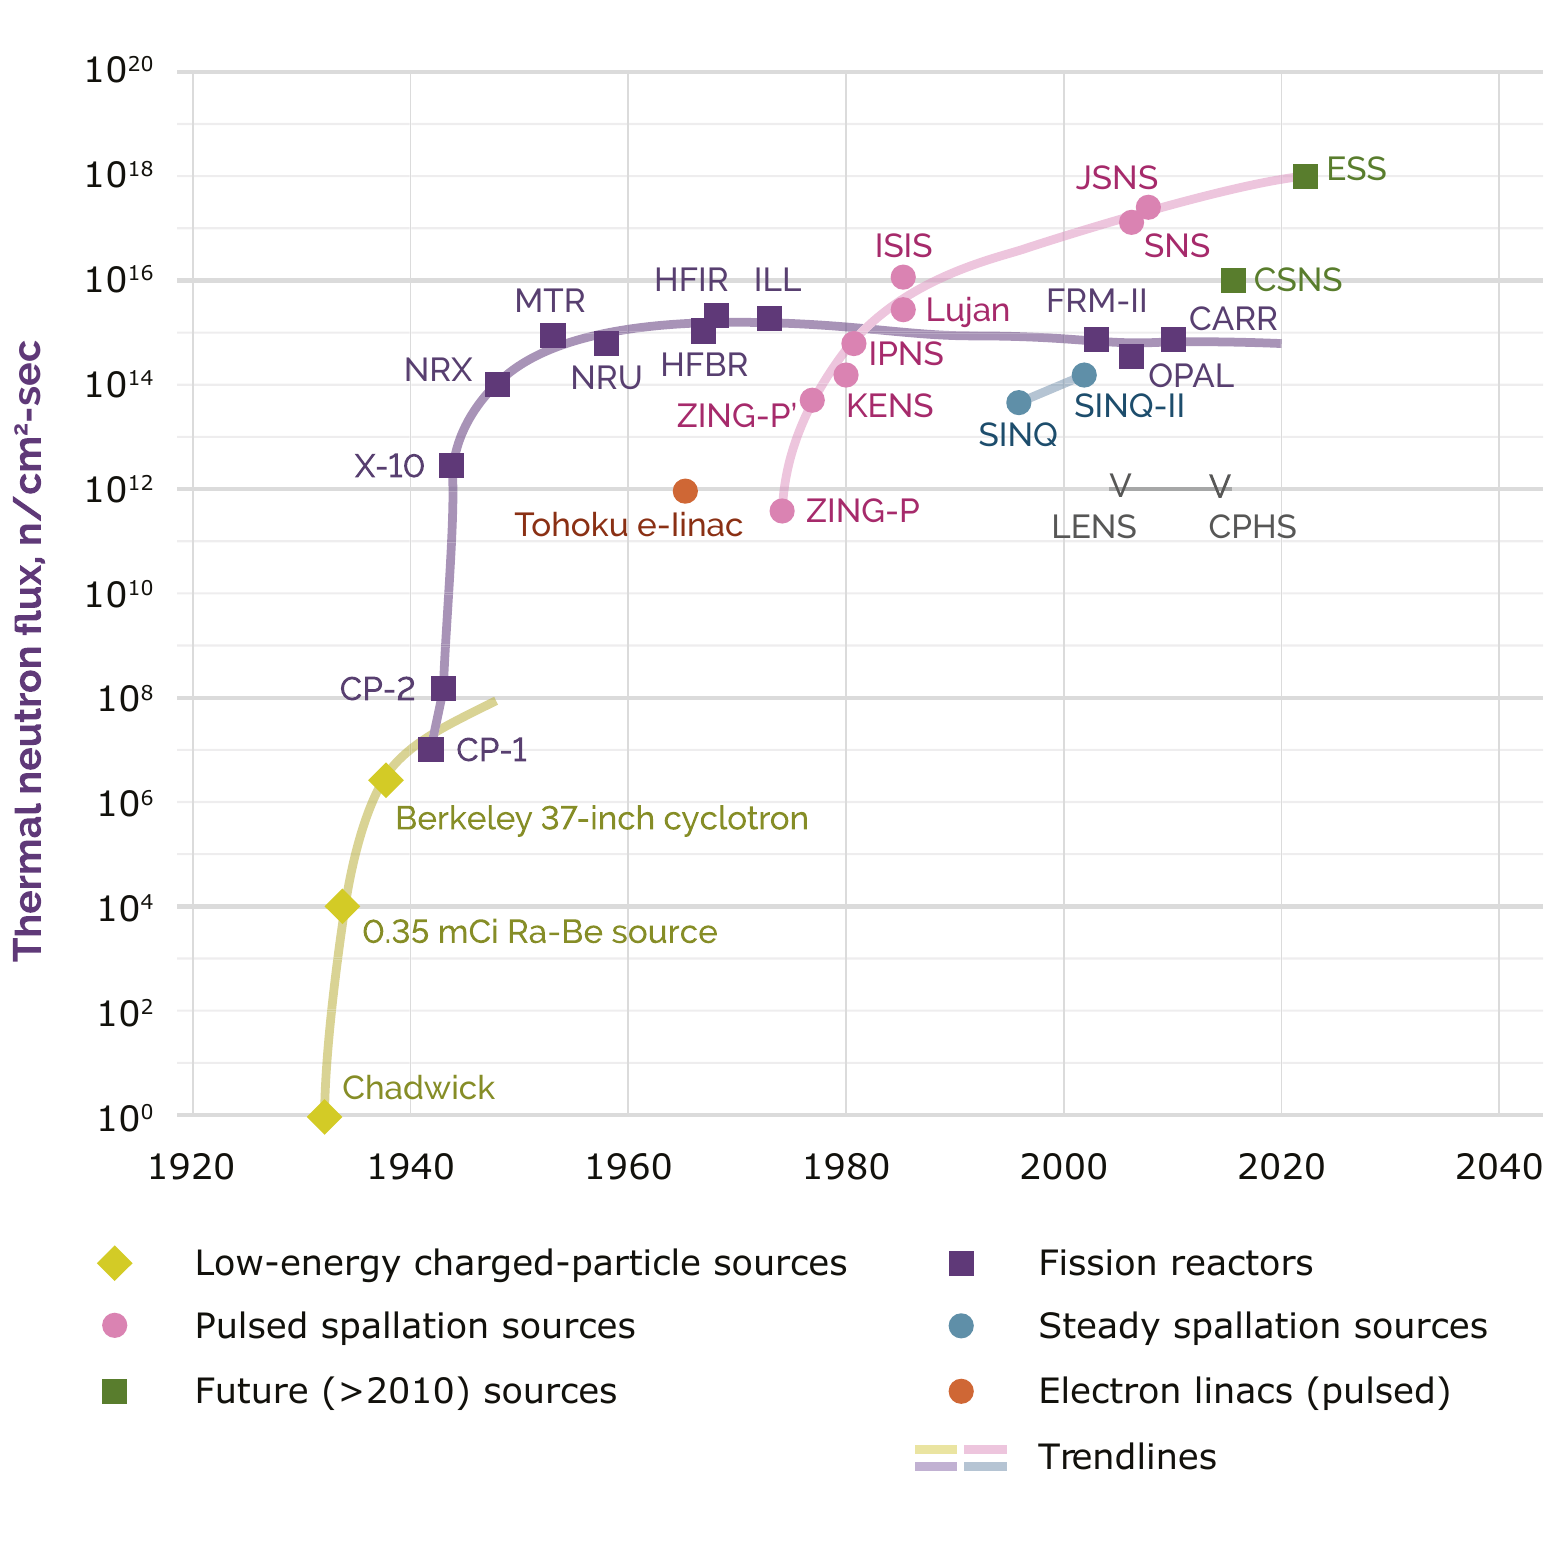
\includegraphics[width=\textwidth]{01_Introduction/figures/fig000_NeutronSources_a}
		\caption{Evolution of thermal neutron sources.}
		\label{}
	\end{subfigure}
	~
	\begin{subfigure}[t]{0.5\textwidth}
		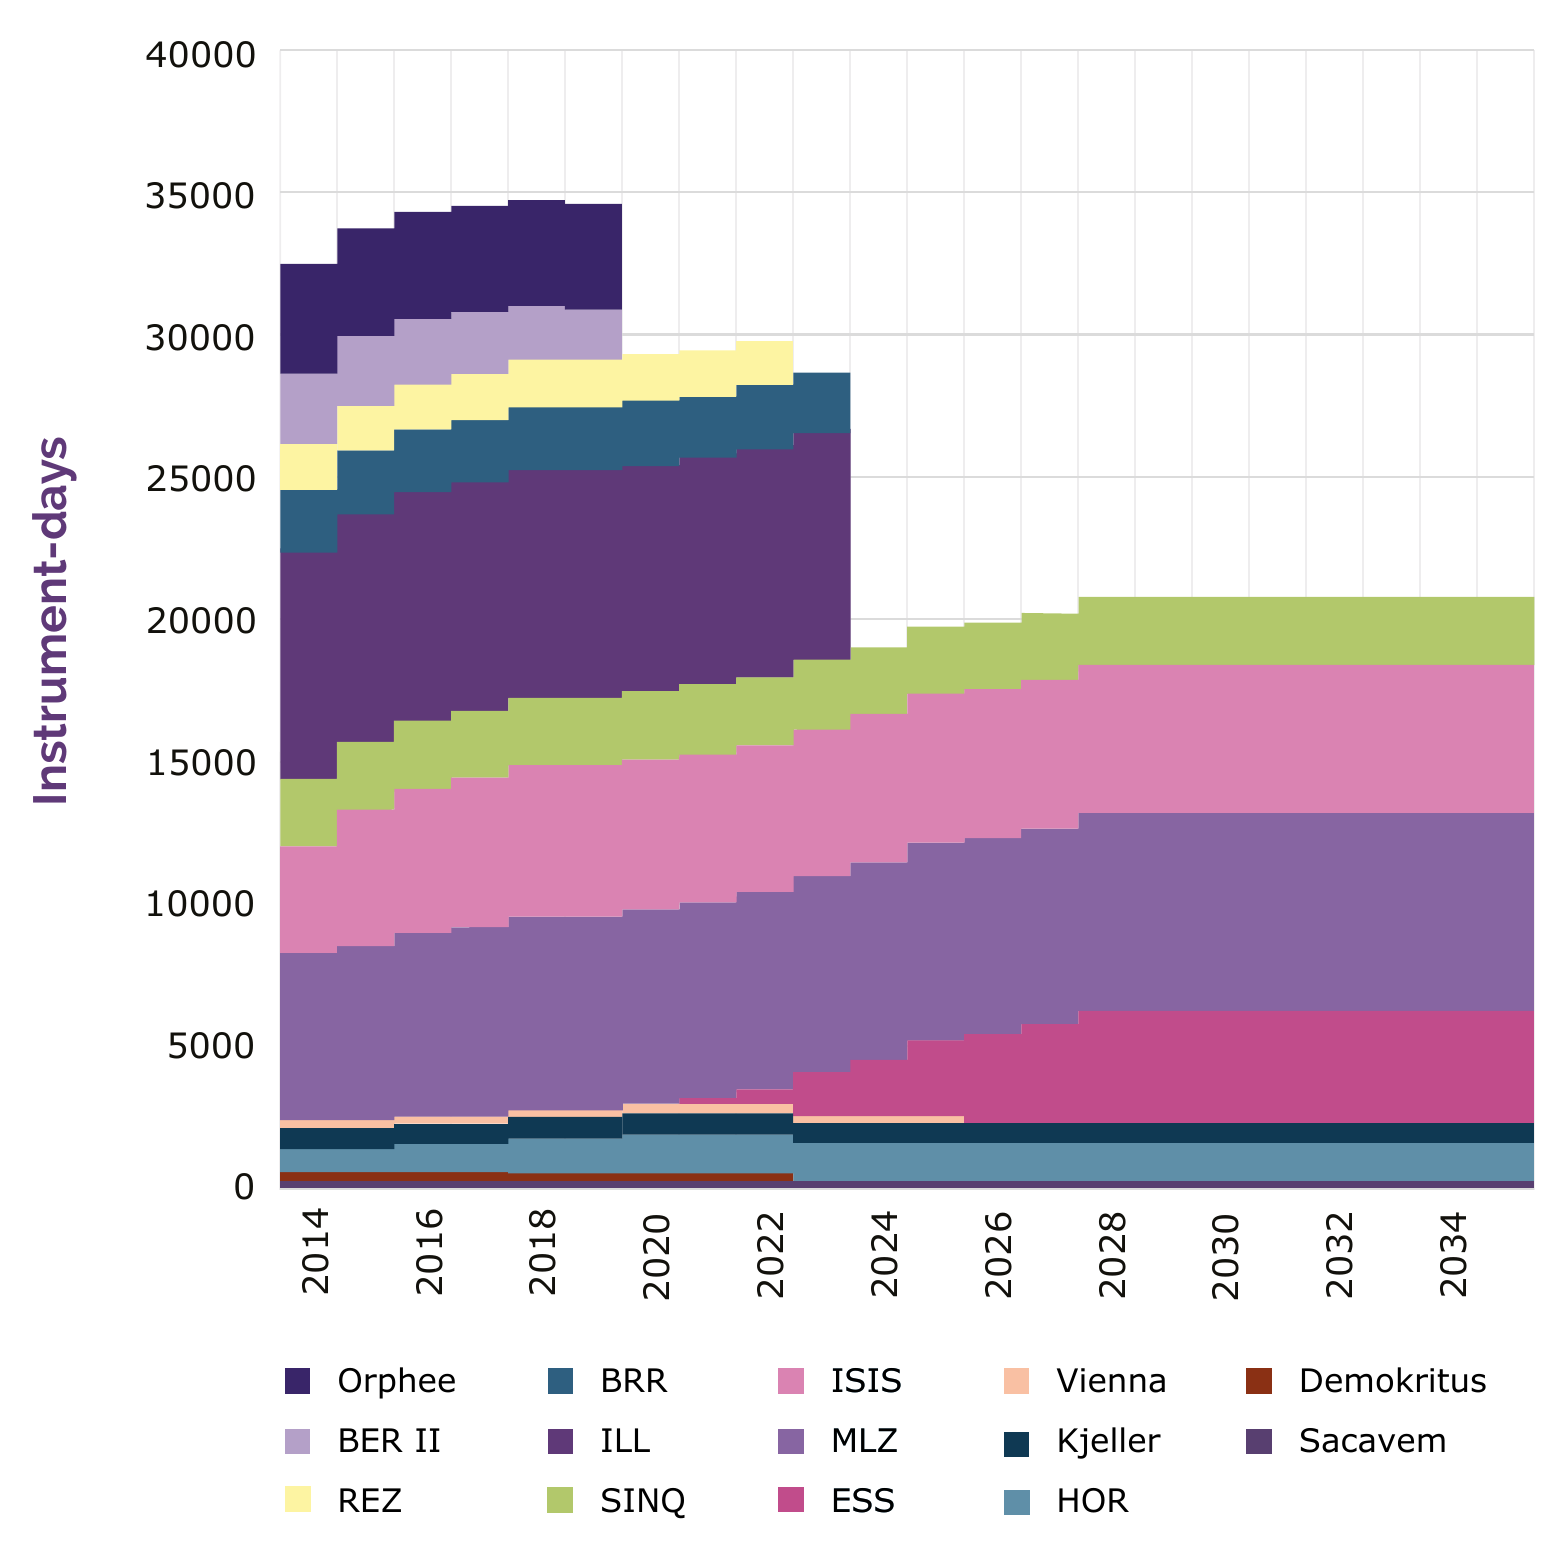
\includegraphics[width=\textwidth]{01_Introduction/figures/fig000_NeutronSources_b}
		\caption{Evolution of beam time for user considering }
		\label{}
	\end{subfigure}
	\caption[]{}
	\label{chap1:fig:NeutronSources}
\end{figure}


  \cleardoublepage
  \section{Bibliography}

  \printbibliography[heading=subbibliography]
\end{refsection}